\documentclass[border=0mm,svgnames]{standalone}
\usepackage{pgfplots,amsmath}
\usepackage{animate} 
\pgfplotsset{compat=1.8}

\begin{document}
    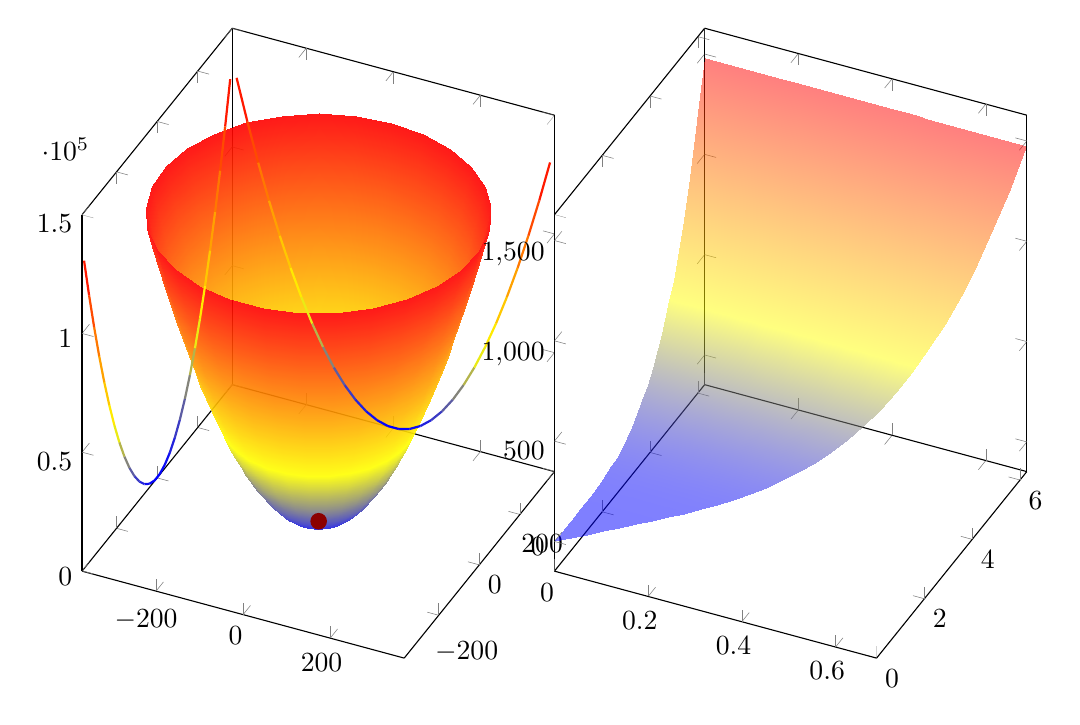
\begin{tikzpicture}
        \begin{axis}[scale only axis,
            name=a1,
            3d box=background,
            height=8cm,
            width=6cm,
            %axis lines=middle,
%            axis on top,
%            axis line style={blue,dashed,thick},
            ymin=-370,ymax=370,
            xmin=-370,xmax=370,
            zmin=-100,zmax=1.5e5,
            samples=30,
            domain=0:360,
        ]

        \addplot3 [surf,shader=interp, z buffer=sort,fill opacity=0.9]
           ({sin(x)*y}, {cos(x)*y}, {(y^2-1)});
           \addplot3[domain=-360:360,samples y = 0, thick,mesh, patch type=line]({x},{370},{(x^2-1)});
           \addplot3[domain=-360:360,samples y = 0, thick,mesh, patch type=line]({-370},{x},{(x^2-1)});        

        \coordinate (ca) at (axis cs:{cos(0)},{sin(0)},0);
        \fill[DarkRed] (ca) circle (3pt);
        \end{axis}

        \begin{axis}[scale only axis,
            at={(a1.north east)},
            anchor=north west,
            3d box=background,
            height=8cm,
            width=6cm,
           domain=0:2*pi,
            %y domain=0:3,
            %xmax=2,zmax=1,
            %domain y=-2:2,
            %axis lines=middle,
%            axis on top,
%            axis line style={blue,dashed,thick},
            % ymin=-370,ymax=370,
            % xmin=-370,xmax=370,
            % zmin=-100,zmax=1.5e5,
            samples=30,
        ]

        \addplot3 [surf,shader=interp, z buffer=sort,fill opacity=0.5]
        ({sin(x)*y}, {cos(x)*y}, {(y^2-1)^2});
        %    \addplot3[domain=-360:360,samples y = 0, thick,mesh, patch type=line]({x},{370},{(x^2-1)});
        %    \addplot3[domain=-360:360,samples y = 0, thick,mesh, patch type=line]({-370},{x},{(x^2-1)});
        

        \end{axis}
    \end{tikzpicture}

\end{document}